\documentclass[12pt]{article}

\renewcommand{\baselinestretch}{2.0}
\usepackage{indentfirst}
\usepackage[a4paper, left=25mm, top=25mm, bottom=25mm, right=25mm]{geometry}
\usepackage{setspace}
\usepackage{tikz-er2}
\usetikzlibrary{positioning}
\usepackage{graphicx}
\graphicspath{{figures/}}

\tikzstyle{every entity} = []
\tikzstyle{every weak entity} = []
\tikzstyle{every attribute} = [node distance=1cm]
\tikzstyle{every relationship} = []
\tikzstyle{every isa} = []

\title{CMPSC 431W Project Proposal\\Phase 1\\Team: Big Leg Carry}
\author{
	Sui, Haojun\\
	\texttt{hzs5220@psu.edu}
	\and
	Deng, Yuanpei\\
	\texttt{dengyuanpei@gmail.com}
	\and
	Zhang, Chenyu\\
	\texttt{dianachenyuzhang@gmail.com}
	\and
	Wang, Hao\\
	\texttt{haowang5128@gmail.com}
	\and
	Chen, Shiqing\\
	\texttt{u0vv0u@gmail.com}
}
\date{\today}


\begin{document}
\maketitle
\thispagestyle{empty}
\newpage
\tableofcontents
\setcounter{page}{1}
\newpage
\listoffigures
\newpage
\listoftables
\newpage

\pagenumbering{gobble}
\pagenumbering{arabic}

\section{Introduction}
\newpage

\section{Requirement Analysis}
\subsection{Sale Items}
The items that we are offering for sale are automobiles. Items listed on our websites are stored in a database management system as an entity. Each item will have a primary key named the item\_id which is unique to every item. As to offer better details to item listings as well as the sake of searching features. Several attributes will be present for the item entity. Some attribute will be visible to the customers as item specifics, and some will be only visible to those who have access to our database as listing specifics. The item specifics include Vehicle Make, Vehicle Condition, Vehicle Model, VIN (Vehicle Identification Number), Year, Mileage, Vehicle Title, Vehicle Type, Body Type, Options, Safety Features, Power Options, Sub Model, Fuel Type, Exterior Color, Interior Color, Drivetrain, For Sale By, Number of Cylinders, Engine Description, Transmission, Trim, and Warranty. On the other hand, the listing specifics indicators include Listing Status, Listing Type, Listing Duration, and Listing Start Time.\par
As most of thse item specifics are very straightforward, some still need further clarification. Vehicle Title refers to the current status of a vehicle, and has two types: clean title and clear title. A clean title is usually used to refer to any car that passes inspection without having any serious physical issues. A clear title is usually used to describe a financial lien that has been placed on a car. For Sale By refers to the type of the seller, which can be either dealer or individual seller. For listing specifics, listing status refers to the status of the listings, and can be active, ended, unsold, sold, and removed. Listing Type can be either auction or buy-it-now. Listing Duration is the time period when the listing is active.

\subsection{Categories}``Shop by Categories" is a necessary way to browse items as customers may not know what to search. The items available at HelloWorld are categorized using a predefined classification tree. Customers will first choose the body type of the vehicle. So the root of the tree will be labeled as ``All Body Type", which we have the nodes of the root as SUV, Pickup Truck, Convertible, Sedan, Crossover, Coupe, Luxury Car, Wagons/Hatchback, Green Cars/Hybrids, Sports Cars, and Minivans/Vans. On the lower levels of the first tree, from top to the bottom, we have: Make, Year, Model, Sub Model, and Trim. \par
An item can be specified by a path through this classification tree. For example, we may
categorize an item as:
\begin{enumerate}
\item SUV $>$ Audi $>$ 2016 $>$ Q7 $>$ Q7 eTron $>$ Base\par
\item All Body Type $>$ Fiat $>$ 2011 $>$ 500 $>$ 500 Abarth\par
\end{enumerate}
\par The depth of the tree varies but is no more than ten levels deep.

\subsection{Suppliers}
In our case, supplier is the car dealer. The attributes of supplier (dealer) are dealer name, address, phone number and rates. The rate is how buyers (user) judge the dealer by several aspects, like customer service, quality of repair, buying process, etc. Dealer will have an inventory. The relation is called owns and the entity is cars. The dealer also has a relation named locates and the entity is address. The reason we choose to make \emph{Address} as an entity instead of an attribute is that we can use the similar schema for registered users. Figure \ref{fig:ERSupp} shows the ER diagram for Suppliers.\\
\begin{figure}[!h]
\caption{ER diagram for Suppliers.\label{fig:ERSupp}}
\begin{center}
\begin{tikzpicture}[node distance=1.5cm, every edge/.style={link}]
	\node[entity] (dealer) {Dealers};
	\node[attribute] (dealername) [left=of dealer] {\key{dname}} edge (dealer);
	\node[attribute] (phone) [above=of dealer] {phone} edge (dealer);
	\node[attribute] (rating) [right=of dealer] {rating} edge (dealer);

	\node[relationship] (owns) [below=of dealer] {Owns} edge (dealer);

	\node[entity] (car) [below=of owns] {Cars} edge (owns);

	\node[relationship] (locates) [below right=of dealer] {Locates} edge (dealer);
	
	\node[entity] (address) [below right=of locates] {Address} edge (locates);
\end{tikzpicture}
\end{center}
\end{figure}

\subsection{Registered Users}
The registered users are the buyers who can buy or bid on an item (car). Buyer must be registered, and identified by a user name and authenticated with a password. When registering, the user must enter the following required information in order to register successfully. These information includes: email address, name, address, phone number and credit card info like type of card, card number, cvv and expiration date. These are the basic information of a registered user. Figure \ref{registered_users} shows how does the interface of registering page look like. (In real design the credit card information will be added.)
\begin{figure}[!h]
\caption{Interface of Registering Page.} \label{registered_users}
\begin{center}
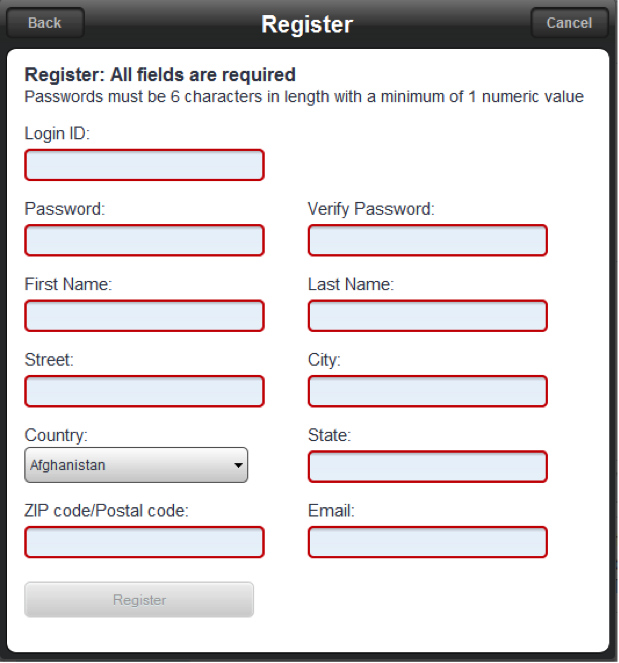
\includegraphics[width=13cm]{registered_users}
\end{center}
\end{figure}
\par In addition, after register a user can complete his whole profile by adding other information like age, gender and annual income. These attributes can be NULL if the user chooses not to fill.

\subsection{Rating}

\subsection{Browsing}

\subsection{Searching}

\subsection{Sale}

\subsection{Bidding}
At HelloWorld, bidding is pretty easy and fair. When seller lists a vehicle on our website, he can choose auction as the listing type. Then he will set a starting price for the auction, a duration, and a reserve price as an optional feature. The starting price has to be greater than 0.99, and lower than the item's buy-it-now price if it has one. The duration can be 3 days, 5 days, and 7 days max. The reserve price which is invisible to buyers is the price threshold where buyers have to bid higher price than the reserve price in order to win the item. If no bid achieves the reserve price at the time when the listing ends, then the item isn't sold. Seller can't change an auction type listing to fixed price listing, but he may end an auction earlier than the projected end time. Seller can change a fixed price listing to an auction type at any time before the end of the listing period, and then the auction duration will be added to the listing upon a successful change from fixed price to auction. To maintain the fairness of the auction, bidders are anonymous to sellers, only the highest bid is visible to the seller. \par
On the buyer side, one can bid on any item at any time, and the number of bids is unlimited. There are two types of bids, one is a one-click-bid, and the other is a max-bid. A one-click-bid is the bid which is one bid increment higher than the current bidding price. The bid increment is determined by the range of current bidding price. Table \ref{pricebid} shows the current bid increment.
\begin{table}[!h]
\caption{Current Price Bid Increment}\label{pricebid}
\begin{center}
\begin{tabular}{|l|c|}
\hline
Price Range(\$) & Bid Increment(\$)\\ \hline
Up to 99.99 & 5\\ \hline
100 to 999.99 & 25\\ \hline
1000 to 4999.99 & 50\\ \hline
5000 to 9999.99 & 100\\ \hline
10000 to 49999.99 & 200\\ \hline
50000 or more & 500\\ \hline
\end{tabular}
\end{center}
\end{table}
\par The max bid is the maximum price a buyer is willing to pay for the item. The max bid is required to be at least one bid increment higher than the current price. When a buyer placed a max bid on an item, the current bid will raise only one bid increment. Buyer can raise the max bid any time during the auction. All the one-click-bids are visible to all the buyers, but max bids are only visible to the buyer who placed it. Buyer can retract his bid any time during the auction, and only if the bid is the highest bid at the moment, but leaving a record of retraction. After retraction, the highest bid placed by other buyer will be the current bid. When buyer A places a bid higher than the current bidding price, buyer B with that bid will be outbid, which means the buyer B will have to bid higher in order to win the item. If buyer B has a max bid, then the bid from buyer A may not be high enough to compete, then buyer A will be automatically outbid with a bid increment at the current bidding range. Buyer A will then place higher bids until the highest bid is lower than his max bid. The highest bid at the end of auction is called a winning bid, the buyer who placed the bid will be the winner of the auction. However, if the highest bid isn't higher than the reserve price, then the buyer isn't winning.

\subsection{Order and Sale Reports}

\subsection{Delivery}

\newpage

\section{Conceptual Design}
\newpage

\end{document}